%%%%%%%%%%%%%%%%%%%%%%%%%%%%%%%%%%%%%%%%%%%%%%%%%%%%%%%%%%%%%%%%%%%
% The following document uses the KOMA Script class
% see http://www.komascript.de/ for more information
%%%%%%%%%%%%%%%%%%%%%%%%%%%%%%%%%%%%%%%%%%%%%%%%%%%%%%%%%%%%%%%%%%%

\documentclass[a4paper,12pt,twoside,BCOR=15mm,parskip=half*]{scrartcl}

\usepackage[utf8]{inputenc} % for directly inserting umlauts etc.
                            % need to store all files as UTF 8 /!\

%%%%%%%%%%%%%%%%%%%%%%%%%%%%%%%%%%%%%%%%%%%%%%%%%%%%%%%%%%%%%%%%%%%
% Please insert your group's details below
%%%%%%%%%%%%%%%%%%%%%%%%%%%%%%%%%%%%%%%%%%%%%%%%%%%%%%%%%%%%%%%%%%%

% group name
\def\groupname{A} % replace X by A,B,C,...
\def\groupcontact{Prof.\ Dr.\ G.~Lüttgen}
%\def\groupcontact{Dr.\ A.~Heußner}

% first group member
\def\AName{Frank Keßler}
\def\AMatrikel{1742945}
\def\AStudSem{SoSySc/4}


% second group member
\def\BName{Andreas Köllner}
\def\BMatrikel{17420191}
\def\BStudSem{AI/7}

% third group member
\def\CName{Jan Martin}
\def\CMatrikel{1796943}
\def\CStudSem{AI/5}


% fourth group member
\def\DName{Simon Meyer}
\def\DMatrikel{1785554}
\def\DStudSem{WI/5}

% fifth group member
\def\EName{Tobias Schwartz}
\def\EMatrikel{1738195}
\def\EStudSem{SoSySc/6}




%%%%%%%%%%%%%%%%%%%%%%%%%%%%%%%%%%%%%%%%%%%%%%%%%%%%%%%%%%%%%%%%%%%
% adapt the following only if needed !

%\usepackage[ngerman]{babel} % change to German spelling etc.

\usepackage[T1]{fontenc}
\usepackage{graphicx}
\usepackage{hyperref}
% For images and other stuff to stop floating by using [H]
\usepackage{float}
%For sidewaysfigure
\usepackage{graphicx}
\usepackage{rotating}

\bibliographystyle{alpha}

% Definition of headings
\usepackage[headsepline]{scrpage2}
\pagestyle{scrheadings}
\clearscrheadfoot
\automark[section]{section}
\ohead{\headmark}
\ofoot{\thepage}
\ifoot{Group \groupname}


%%%%%%%%%%%%%%%%%%%%%%%%%%%%%%%%%%%%%%%%%%%%%%%%%%%%%%%%%%%%%%%%%%%
% main document

\begin{document}

\pagestyle{empty} % temporary change to pagestyle without headings and footers

\includegraphics[width=4cm]{logo}\hfill

\includegraphics[width=6.5cm]{uni-bamberg-logo-de}\\
\section*{\centering Guidelines for the SWT-SWL-B Report}
\centering\emph{Prof.\ Dr.\ Gerald Lüttgen ~\textperiodcentered~  Ms. Ons 
Seddiki, M.Sc. \\ Winter Semester 2016/17}

\vfill
\flushleft
\subsubsection*{Language}
The report shall be written in English or German.

\subsubsection*{Format}

The report shall be printed on A4 paper, use a double-sided, single-spacing page format with reasonable margins (at least~15mm and at most~30mm to the left and right) and employ font \emph{Computer Modern} or \emph{Times} in size~12pt. All pages shall be numbered.

\subsubsection*{Structure \& Content}
The report's structure shall be the one of this document. In particular, the report shall contain a title page, a table of contents, a list of figures, all sections and subsections of this document, a bibliography, and an appendix with the final product backlog.  Further appendices may be added as needed.

In the sequel, the expected content of each section is summarized in italics.  It is strongly recommended that you use this document's {\LaTeX} sources as a template for your group's report.

\subsubsection*{Expected Number of Pages}
The report shall be 30--50~pages \emph{of text} in length.  This excludes the title page, the table of contents, the table of figures, the bibliography, all appendices and the Eh\-ren\-wört\-liche Er\-klä\-rung, as well as all figures, diagrams and code excerpts/listings.







\subsubsection*{Figures \& Diagrams}
Each figure, diagram or code excerpt/listing/table shall be easily readable and have a number and caption that also appears in the list of figures/tables. See Figure~\ref{fig:example} and Table~\ref{tab:example} as examples.



\begin{figure}[h]
  \centering
  
\includegraphics[width=3cm]{logo}
  \caption{Example figure.}
  \label{fig:example}
\end{figure}

\begin{table}[h]
  \centering
  \caption{Example table}
  \begin{tabular}{l||c|c|c|c|c|c}
    Section number & 1 & 2 & 3 & 4 & 5 & 6\\
    \hline
  Expected. no. of pages & 2--3 & 6--12 & 5--8 & 10--15 & 4--7 &3--5\\
  \end{tabular}
  \label{tab:example}
\end{table}

\subsubsection*{References}
Citations shall be marked in square brackets by an alphanumeric author-year system, e.g., \cite{scrumbook,userstories} and \cite{texbook}. Make sure that all sources are referenced properly and all bibliography entries are complete.


\subsubsection*{Ehrenwörtliche Erklärung}
All group members shall sign the \emph{Ehrenwörtliche Erklärung} (Declaration of Proper Academic Conduct) on the report's last page.



%\subsubsection*{Mark Allocation}
%
%\begin{tabular}{|l||c|c|c|c|c|c|c||c|}
%  \hline
%  Section & General & Project & Reqs. & Arch.\& D. & Realiz. & QA & Review & \ \ $\sum$\ \ \\
%  \hline
%  Marks & 15 & 30 & 60 & 80 & 105 & 70 & 40 & 400 \\
%  \hline
%\end{tabular}

\vspace{10ex}

\textbf{Please do not forget to justify in your report all technical and non-technical aspects of your group's conduct of the software development project.}




\cleardoublepage
\setcounter{page}{1} % reset page numbers to restart from one
\pagestyle{scrheadings} % turn back to normal headings
 % just comment this line in your final version

\begin{titlepage}
\thispagestyle{empty}
{\sffamily

\includegraphics[width=4cm]{logo}\hfill

\includegraphics[width=6.5cm]{uni-bamberg-logo-de}\\
\vspace*{2cm}
\begin{center}
	\bfseries
  \LARGE Report\\[1.5ex]
  SWT-SWL-B Software Engineering Lab\\[1.5ex]
  Winter Semester 2016/17
\end{center}
\vspace{1cm}
\begin{center}

	{\Large\bfseries Group \groupname\\[5mm]}

	\begin{tabular}{lll}

    \AName & \AMatrikel &\AStudSem\\[3mm]
    \BName & \BMatrikel &\BStudSem\\[3mm]
    \CName & \CMatrikel &\CStudSem\\[3mm]
    \DName & \DMatrikel &\DStudSem\\[3mm]
    \EName & \EMatrikel &\EStudSem\\[3mm]
    \FName & \FMatrikel &\FStudSem\\[3mm]

	\end{tabular}\\[1cm]

    Supervisor: \groupcontact\\[2ex]

    Version: \today
\end{center}
}
\end{titlepage}




\cleardoubleemptypage
\tableofcontents

\clearpage
\listoffigures
\listoftables

\clearpage
\section{Project Organization}
\flushleft
In this section we describe the overall goal of the project, the internal organisation and work distribution of our group, and our activities during the Blast-off of the project.  \\

\subsection{Goal of the Software}

In this subsection we describe the goal of the Test Data Analyser (TDA). The TDA is developed for medatixx GmbH \& Co. KG, a company that develops software for medical practices. TDA is an application to help software developers and testers at medatixx to analyse test data of their software. Purpose, advantage, and measurement are the three parts of which the goal of TDA is made of. \\
\ \\
\large\textbf{Purpose}\\ 
During the development of their software, medatixx uses a sequence of builds, i.e. (pre-)release versions of the software. To ensure the quality of their product, each build is tested via a number of unit tests which are defined and executed on the classes of the corresponding build. The collection of these unit tests, their classes and the build they belong to, and their results is called a test run. TDA shall support the analysis of these test runs to help medatixx to discover builds with classes that are problematic to test. \\ 
To do so, TDA shall extract the necessary information from the test run XML files provided by medatixx, analyse the information in different ways including the usesage of the Apriori algorithm and visualise the results of the information analysis. \\ 
\ \\

\large\textbf{Advantage}\\ 
The TDA provides new and more detailled information on the tests of different builds. It highlights the classes with the highest failure percentage of a specific test run. It shows the evolution of a class by visualising its failure percentages over multiple test runs. By using the Apriori algorithm it shows possible associations between different classes. It offers an easy method to compare the tests of a specific class in different test runs. \\ 
With the additional information the TDA is making available for testers at medatixx, they get new insight into their testing methodology and the overall test quality is improved. \\
\ \\

\large\textbf{Measurement}\\ 
Due to the easily accessible information on test runs and the discovered associations between classes, the resolution of failed classes and their corresponding unit tests will be accelerated by 50 \%. 

%TODO: Find better solution for table
\newpage
\subsection{Organisation of the Group}

\begin{table}[!h]
  \caption{Distribution of work}
  \centering
  \begin{tabular}{p{2cm}||p{4.2cm}|p{4cm}|l|}
    Name & Responsibilities & Principal Artefacts & Work Time\\
    \hline
    \hline
    Andreas & Identify user stories & User story cards & 5 \\
    \hline
    Andreas & Create stakeholder map & stakeholder map & 3 \\ 
    \hline
    Andreas & StAXParser & Methods for parsing & 10 \\ 
    \hline
    Andreas & Preparing paper prototype & Paper prototype & 6 \\
    \hline
    Andreas & Create high level architecture diagram & High level architechture diagram & 4 \\ 
    \hline
    Andreas & Documenting Sprint 2 & Sprint 2 wiki & 3 \\ 
    \hline 
    Andreas & Directory browser in GUI & Corresponding methods & 3 \\ 
    \hline
    Andreas & Tree view and handling for imported test runs & Corresponding methods & 11 \\ 
    \hline
    Andreas & Testing of classes in package logic without Parser, Analyzer & JUnit tests & 12 \\ 
    \hline 
    Andreas & Create use case diagram & use case diagram & 7 \\ 
    \hline
    Andreas & Exception handling in StAXParser & Corresponding methods & 2 \\ 
    \hline
    Andreas & Documentation of Model & Javadoc in Model & 2 \\ 
    \hline
    Andreas & Documentation of Logic classes & Javadoc in Logic & 8 \\ 
    \hline
    Andreas & Author of chapter 1 & Chapter in project report & 10 \\ 
    \hline
    Andreas & Author of chapter 4.1 & Chapter in project report & 3 \\ 
    \hline
    Andreas & Author of chapter 4.2 & Chapter in project report & 12 \\
    \hline
    \hline 
    \textbf{Total \newline Andreas} & & & \textbf{total}   \\
    \hline
    \hline
  \end{tabular}
\end{table}

\subsection{Project Blast-off}

The Project Blast-off is the most important activity to decide whether or not to go ahead with a project. It is used to gather information on the project and make sure that it is viable and well founded. \\ 
Before we defined our goal for the project, we agreed that every member of our group should read and understand the project brief until our first official meeting. In our first meeting we collectively went through the requirements and every single described scenario. After making sure we were all on the same page and understood the content, we defined our goal of the whole project as described in subsection 1.1. \\ 
We continued by going through it again and highlighting epics and first user stories. In further cycles we worked on detailing them and lastly started on finding adequate tasks for the now written cards. Those tasks were not yet assigned to individual persons, as we still wanted to have the option to allocate them according to one’s time and knowledge on the described topic later on. Soon first challenges arose when it came down to connecting tasks with one adequate user story. It appears that some tasks are used for many user stories, because they describe core functionalities and therefore have to be implemented in order to make the rest working. Then again, sometimes it was just difficult to assign a specific task to a user story at all, because it described a mandatory functionality that just wasn’t covered by any adequate user story and creating one seemed not to be possible. We decided to discuss our concerns in the first meeting with the client.\\ 
During further discussion we identified the stakeholders of the project as shown in the stakeholder map in figure \ref{StakeMap}. \\

\begin{figure}[h]
\begin{center}
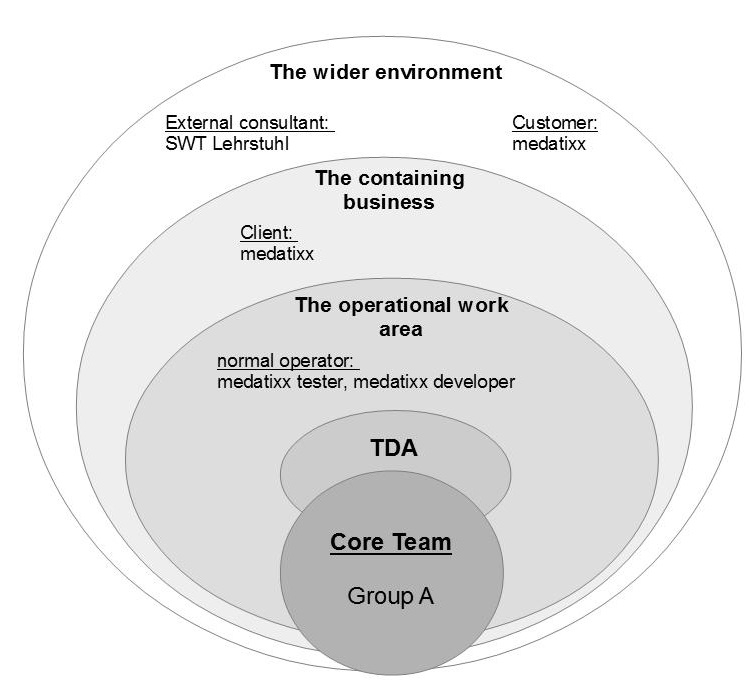
\includegraphics[scale=0.5]{pics/StakeMap2.jpg}
\caption{Stakeholder map}
\label{StakeMap}
\end{center}
\end{figure}

As you can see in figure \ref{StakeMap} medatixx GmbH \& Co. KG is listed as customer and client, since they use the TDA as an inhouse application. The typical users or normal operators of TDA are software testers and developers at medatixx. \\ 
In the next step we thought about the boundaries of our system, i.e. the scope of the work. As shown in figure \ref{Scope}, the TDA only has one indirect interface to adjacent systems. That interface is used by medatixx to provide the XML files from which TDA extracts the necessary information. We visualised this connection in the following context diagram. \\

\begin{figure}[h]
\begin{center}
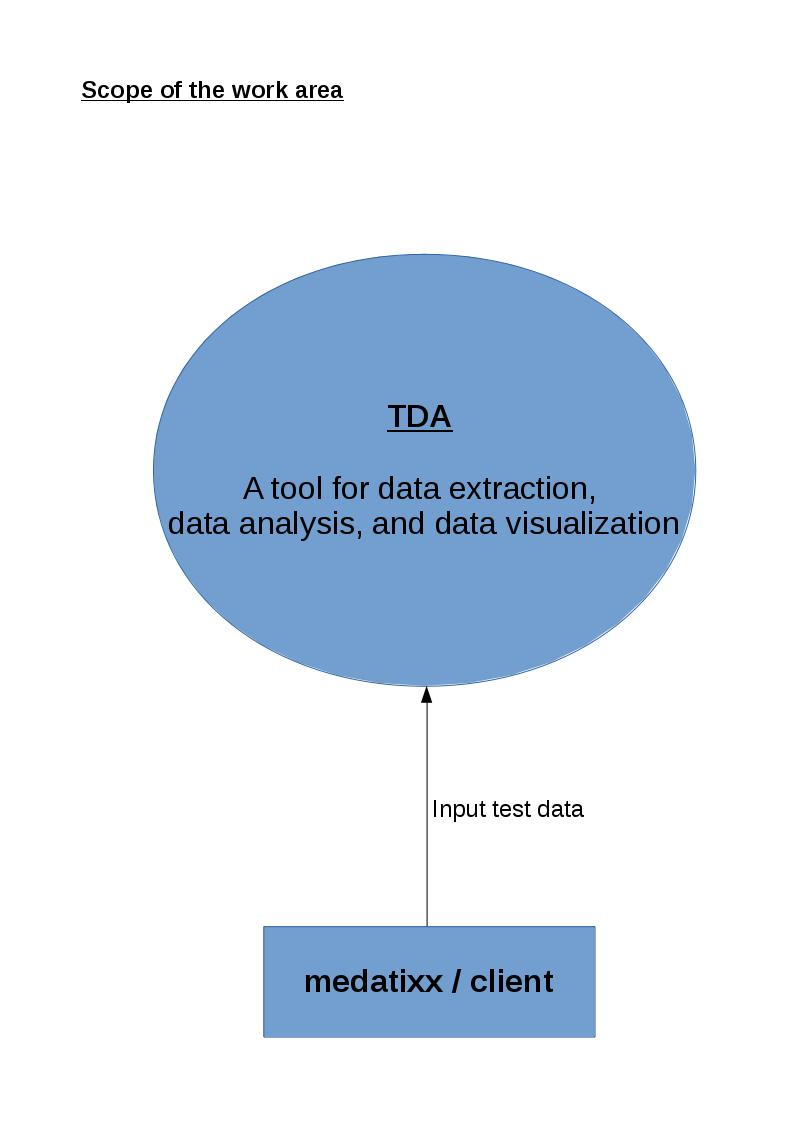
\includegraphics[scale=0.2]{pics/Scope_of_Work_Context_Diagram_v2.jpg}
\caption{Context diagram} 
\label{Scope}
\end{center}
\end{figure}

After we defined the scope of work of the TDA we discussed which architecture and design patterns we could use for our system. Also first ideas for specific classes and interfaces arose. Gladly, all of us had already visited the DSG-AJP-B course in previous semesters and so we could all contribute equally to the discussion without too much additional explanation of any named techniques. Since we have to deliver a GUI application in Java, we decided on a standard model-view-controller pattern. The corresponding high level architecture diagram is shown below in figure \ref{HLA}. \\

\begin{figure}[h]
\begin{center}
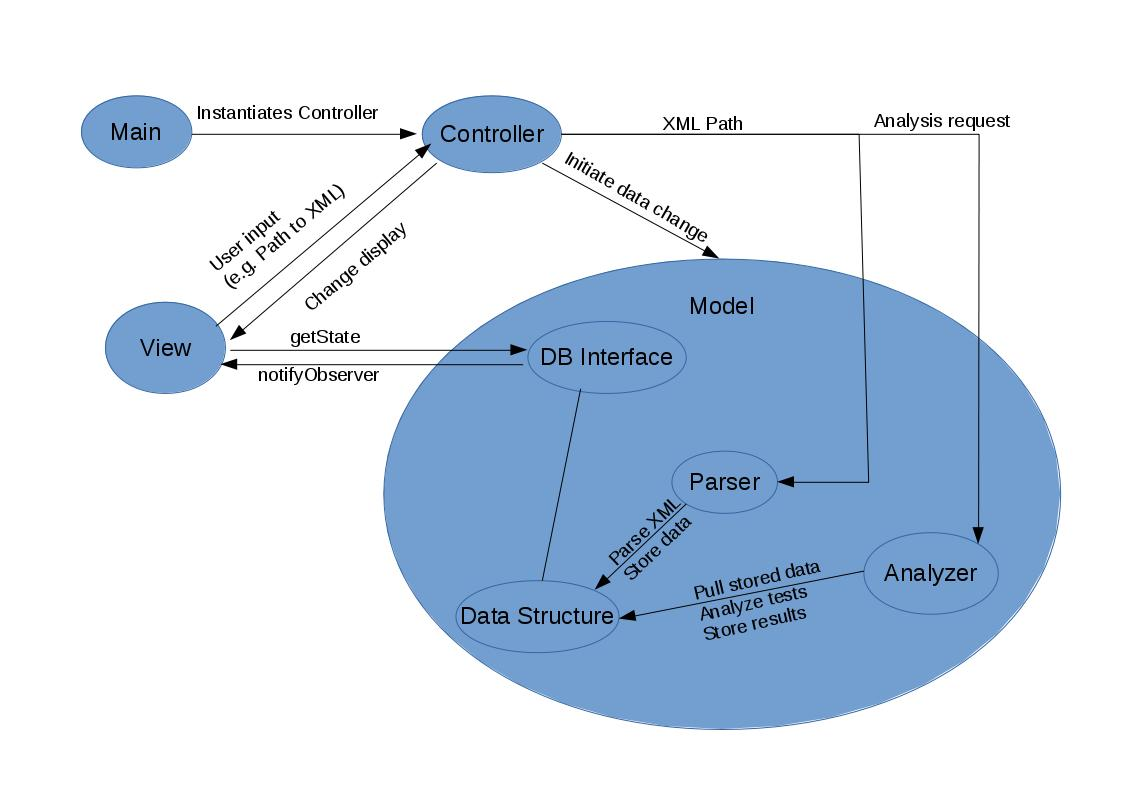
\includegraphics[scale=0.3]{pics/Architecture_diagram.jpg}
\caption{High level architecture} 
\label{HLA}
\end{center}
\end{figure}

In the next step we constructed a central glossary to minimize misunderstandings in our communication and make sure to understand the language of the client. \\ 

\begin{table}[h]
  \caption{Glossary}
  \label{Glossary}
  \centering
  \begin{tabular}{p{2.3cm}||p{10cm}|}
  	Term & Meaning \\ 
  	\hline
  	\hline
  	Test run & A collection of unit tests of one specific build \\ 
  	\hline
  	Failure percentage & Failure percentage of class C = (Number of failed unit tests for class C) / (Total number of unit tests for class C) \\ 
  	\hline
  	TDA & Test Data Analyser (the program to be developed) \\ 
  	\hline
  	Problematic class & Class with a high test failure percentage \\ 
  	\hline
  \end{tabular}
\end{table}

The last task of sprint 0 was to conduct a risk analysis. Most likely we have to deal with sickness of individual persons every now and then. We try to limit the impact of this by good group communication, shared responsibilities and documentation. Also it is likely that the client changes the specifications along the way, what we’re going to cope by building adaptable software with loose coupling and high cohesion. The risks with the highest impact would be someone leaving the project or the complete loss of all our data. We are going to deal with this with shared responsibilities and backups, respectively. A complete and detailed risk analysis is shown in table \ref{Risks}. \\ 

\begin{table}[h]
  \caption{Risk analysis}
  \label{Risks}
  \centering
  \begin{tabular}{p{3cm}||p{5cm}|p{2cm}|p{2cm}|}
  	Risk & Coping & Likelyhood & Impact \\ 
  	\hline
  	\hline
  	Someone leaves the project & Shared Responsibilities & <10\% & Severe \\ 
  	\hline
  	Complete data loss & Back ups & 5\% & Severe \\ 
  	\hline
  	Usage of prohibited packages & Regular checks, test on external IDE & 10\% & High \\ 
  	\hline
  	Sick team member & Shared responsibility, documentation & 50\% & Medium \\ 
  	\hline
  	Client changes specifications & Adaptable software (loose coupling \& high cohesion & 50\% & Medium \\
  	\hline
  	Unprecise specification (missing examples) & Communication with client & 20\% & Medium \\ 
  	\hline
  	Research stories far more complex than expected & Do research early, conservative planning & 5\% & Medium \\ 
  	\hline
  	Differing visions (unnecessary development) & Refular internal communication & 30\% & Medium \\ 
  	\hline
  	Lab PCs insufficient for testing/development & Write performant code & 5\% & Low \\ 
  	\hline
  \end{tabular}
\end{table}

\clearpage
\section{Requirements}
%\flushleft

\begin{table}[!h]
  \caption{List of user stories}
  \centering
  \begin{tabular}{l||l|l|l|l|}
    ID & Name & Size &  Source & Sprint\\
    \hline
    R1&Research Apriori&Medium&Project brief&1\\
    R2&Research StAX Parser&Small&Project brief&1\\
    1&Testing&Medium&Project brief&5\\
    2&Imports in tree structure&Medium&Client&2\\ %Original ID was 2.001; 
    3&Testrun chart&Medium&Project brief&3\\
    7&Testrun table&Medium&Project brief&2\\
    8&Association Analysis&Large&Project brief&3\\
    9&Testrun Selection&Medium&Project brief&2\\
    12&Store XML in classes&Medium&Assumed by us&1\\ 
    18&XMLParsing&Medium&Project brief&1\\
    23&Implement Apriori Algorithm&Large&Project brief&4\\
    24&Display Analysis Data&Medium&Project brief&4\\
    25&Additional usage scenario&Medium&Project brief&5\\
    26&Code Documentation&Small&Project brief&5\\
    27&Distribution with suited license&Small&Project brief&5\\ %not sure about origin of 27/28
    28&Creating a help function&Small&Project brief&5\\
    213&Evolution of a class&Large&Assumed by us&4\\ 
  
	\end{tabular}
  \label{tab:user_stories}
\end{table}

As you may notice our user stories have quite strange IDs with a lot of numbers missing in between. This is because in the beginning we wanted to prevent that the IDs indicate an order. Retrospectively, we came to the conclusion that this was a mistake, as it caused more confusion in our group.\\
In the end we tried to fix this a little bit (user stories 23-28), however, the project was already quite far in progress, so the majority of user stories still has random IDs.  \\
\newline
In Sprint 0 we discussed the content of the project brief and to make sure we all were on the same page we proceeded to draw a first use case diagram. This was helpful in multiple ways, as it gave us an overview over the whole project in addition to helping us figure out functional requirements.\\
The use case diagram was always maintained when we received new requirements from the client or we changed our code in such way that we had to update the diagram. Thanks to this progress, we for example came to the conclusion that a start screen where you can select xml-files makes a lot of sense, since all features depend on data, which has to be parsed first.

\begin{sidewaysfigure}
	\begin{center}
		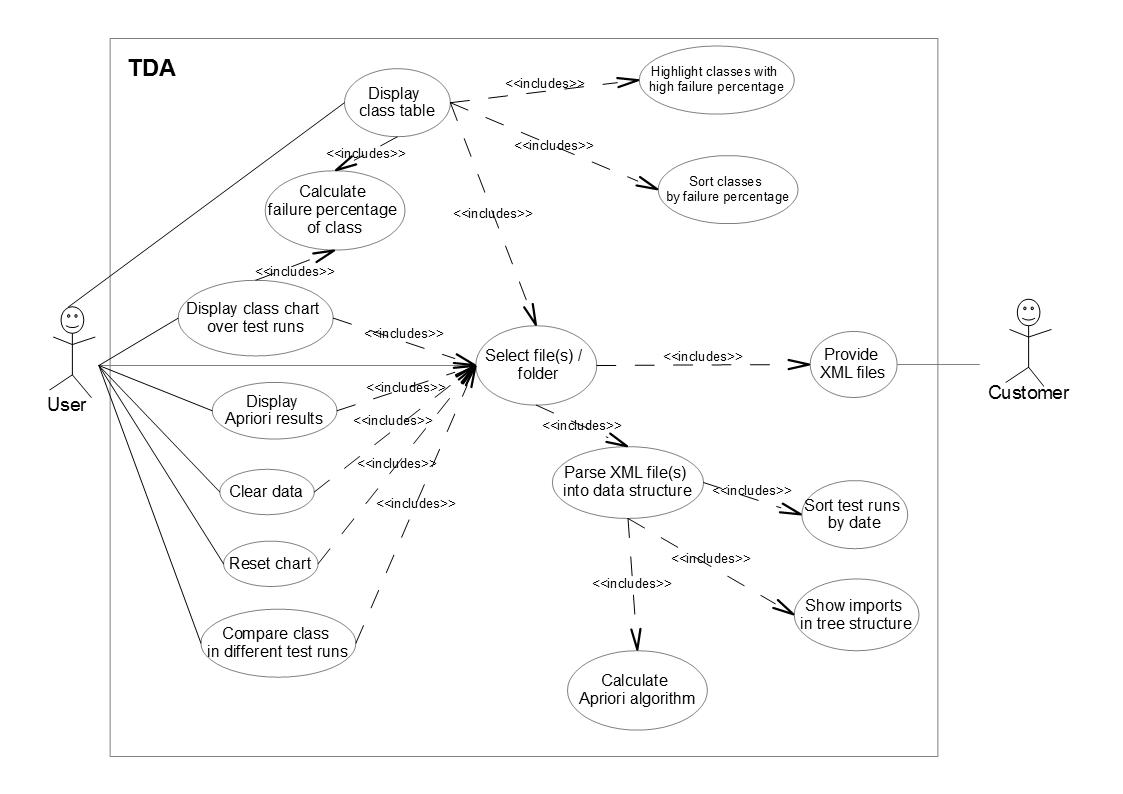
\includegraphics[scale=0.6]{pics/UseCaseDiagram.jpg}
		\caption{Use case diagram}
		\label{use-case}
	\end{center}	
\end{sidewaysfigure}
Based on this use case diagram \ref{use-case} we then proceeded to write user stories and corresponding tasks. This way we always had the requirements in eye-sight on the task-board.

\subsection{Requirements derived from project brief}
\subsubsection{Functional requirements}
\begin{itemize}	
	\item A table shall show all tested classes of one testrun\\
	Fit criteria: testruns ordered descending by failure percentage and highlight red if failure percentage is higher than 75\% and yellow if it's between 50 and 75\% 
	\item A chart shall display the change of a specific class over all parsed testruns\\
	Fit criteria: every class can be added to chart only once - not multiple times; Is good readable even with a lot of testruns
	\item Association analysis shall use the well-established Apriori algorithm\\
	Fit criteria: Strong rules are generated from frequent item sets
	\item XML-files shall be parsed using the StAX parser\\
	Fit criteria: Every correct xml-file will be read and stored in our data structure
	\item The user shall be able to select a specific testrun to get more information\\
	Fit criteria: When testrun is selected the table and all relevant testrun details will be shown.
	\item The association analysis output shall be displayed in a convenient way.\\
	Fit criteria: It visualizes the output in an easy, but contentful way, which is approved by the client.
	\item Two more usage scenarios shall be suggested to the client and implemented\\
	Fit criteria: Scenarios are accepted by the client and implemented to his wishes
	\item The software shall be distributed with a suited open-source licence\\
	Fit criteria: Licence shall be visible from within the software and be free("libre")
	\item A manual shall be accessible from within the software\\
	Fit criteria: Explains all features and how they are used
\end{itemize}

\subsubsection{Non-Functional requirements}
\begin{itemize}
	\item All features shall be tested sufficiently\\
	Fit criteria: Coverage of at least 90\%
	\item Source code shall be documented properly\\
	Fit criteria: Every class is documented according to the project brief
\end{itemize}

\subsubsection{Development constraints}
\begin{itemize}
	\item The software has to run on a standard SWT-lab PC
	\item Software shall be implemented in Java; documented using Jdoc; tested with JUnit;
	\item Copied code shall be cited with its source
	\item Development shall be done via the SWT-Git-repository
	\item Commit messages shall have the following format: \\
	SPRINT n SUBSTANTIAL m \\
	documentation of commit \\
	full name of responsible person
	\item The file structure shall be as follows:
	\begin{itemize}
		\item 'src' containing source files
		\item 'test' containing JUnit tests
		\item 'doc' containing JavaDoc of the sources
		\item 'uml' containing UML-diagram files
	\end{itemize}
	\item Final release shall look as follows:
	\begin{itemize}
		\item source files; unit tests; Jdoc
		\item binary release (jar)
		\item project report
	\end{itemize}
	
\end{itemize}
\subsection{Requirements assumed by us}
\subsubsection{Functional requirements}
\begin{itemize}
	\item The class overview in the sidebar shall display all classes in a tree structure\\
	Fit criteria: classes are in a tree based on packet structure and clicking on them inserts them in the chart
	\item All relevant data from the xml-files shall be stored in corresponding classes(data structure)\\
	Fit criteria: all unit tests on the data structure pass
	\item The user shall be able to compare two specific testruns of one class with respect to its unit tests.\\
	Fit criteria: Not possible to compare different classes; Shows all passed and failed unit tests and the difference between two runs
\end{itemize}

\subsubsection{Non-functional requirements}
\begin{itemize}
	\item The software shall run reliably\\
	Fit criteria: Shall maintain a 95\%+ uptime
	\item Parsing and computing shall be reasonable fast with respect to the amount of files parsed\\
	Fit criteria: Should not take longer than 2 minutes for 1000 files
	\item The parser shall only parse xml-files with the correct format\\
	Fit criteria: When a wrong format is detected an exception shall be thrown
\end{itemize}
\subsection{Requirements added by client}
\subsubsection{Functional requirements}

\begin{itemize}

%Sprint 1:
\item choose a folder and parse all containing XML files in the folder and its subdirectory\\
Fit criteria: every *.xml file is parsed and added to the data structure

%Sprint 2:
%Maybe NFR:
\item Table: classes with failure percentages between 50 - 75\% should be highlighted yellow and failure percentages between 75 - 100\% should be highlighted red; it should be possible to hide/show all classes with a failure percentage of 0\%\\
Fit criteria: The table highlights the classes correctly according to failure percentage
\item Failure percentages in table should be rounded to 2 decimals\\
Fit criteria: All percentages are rounded correctly
\item Testrun totals: a note, stating that not all totals of the testrun are shown above the table should be visible; a button shall enable the user to see all totals\\
Fit criteria: All relevant information is displayed, when the details button is pressed

%Sprint 3:
\item one click in tree sidebars for selecting files (no doubleclick)\\
Fit criteria: Only one click is needed to select testruns or classes
\item hover over chart entries shall show testrun information\\
Fit criteria: On hover the start time and the number of failed/passed unit tests shall be displayed
\item chart shall have its own page instead of being shown in the main window below the class table\\
Fit criteria: the chart shall not be under the table anymore, so it has more space to display data
\item The functions to filter the Apriori results by confidence and distance should be implemented\\
Fit criteria: Correct filtering of confidence and by distance shall be possible

\item A second additional usage scenario should be proposed, but due to the given point in time the focus should be to finalize the already implemented functionality\\
Fit criteria: The scenario is presented to the client and accepted


Fit criteria: 

\end{itemize}

\subsubsection{Non-functional requirements}
\begin{itemize}
%Sprint 2:
\item The software shall load most of its data in the beginning, so you can use the tool without waiting times later on\\
Fit criteria: When switching between features there shall be minimal loading times if at all



\item program shall adapt its layout automatically to lower resolutions or resizing\\
Fit criteria: The content is always well readable, no matter the resolution or display size
%Sprint 4:
%NFR
\item The outcome of the Apriori algorithm should be visualized in a better way, since the two tables are not easy to read.\\
Fit criteria: A easier to understand visualization shall make clear what classes are dependent
\end{itemize}

\clearpage
\section{Architecture \& Design}
%\flushleft
%\emph{(Approx.~5--8~pages of text.) Tobias}
\iffalse
\emph{Describe both the architecture and the design of your 
software. Illustrate its architecture and design using appropriate UML diagrams. 
Motivate its architecture and design in the light of design principles and 
possible alternatives. Also highlight any use of architectural 
patterns and design patterns. Pay special attention to justifying all design 
decisions taken.}
\fi

\subsection{Initial Idea}
At the beginning of the project, the model-view-controller architecture has been chosen to be the basis for the TDA. For this, the project is divided into three different layers, each responsible for a specific functionality. In particular, the business logic is separated from the control and presentation layer. This follows the principle of separation of concerns.

The model-view-controller pattern is defined as a compound pattern. This means that it is a combination of several other design patterns that work together. As the name predicts, it consists of a model, view and controller, which all have different responsibilities. The view is responsible for displaying information and for allowing interaction with the user. The model holds the program's data and executes all related computations. It is the representation of the business logic. Finally, the controller works close with the view and functions as a translator for the interaction between the previously mentioned components. View and controller together build the user interface.
While the model can function on its own, view and controller depend on the existence of a model. This makes the user interface easily changeable or even exchangeable as a whole, without touching the logic at all. In other words, the proposed architecture is also designed for change. Additionally, it is possible to implement multiple views next to each other, all relying on the same underlying logic. The preferred view can then even be displayed at run time and for example based on the machine or device it is being executed on.

Since the TDA shall display all the information in an adequate graphical user interface, this approach seemed to fulfill the criteria and fit our needs. Although there were no concrete plans for implementing an additional user interface, it is always a good practice to be prepared for similar requests that arise later in the project phase.

Also very early in the project development, we discussed how the given XML-files shall be read and whether they shall be processed and stored internally for later, faster processing. Database approaches were discussed and compared to directly loading the information in an internal infrastructure. A detailed description of this process and the final results can be found in section~\ref{sec:data_structures}.
The selected data structure and its location also have a big influence on the selected architecture and the overall class interaction. With the current approach, this clearly was a part of the model.

After other components like the parser and the analyzer were addressed in later project development, the model steadily increased in size and with it in complexity. Other design patterns and architectures were needed, in order to maintain the highly flexible and clearly structured code that we strive to achieve. That's why we changed the high-level architecture, as described in detail in the following paragraph, and used the previously explained model-view-controller pattern only as a subsystem for the new architecture.

\subsection{Final approach}
The high level architecture of the TDA now follows the repository architecture. This design is defined by one central entity and different subsystems that are connected directly to the named system. The central entity hereby usually functions as a data storage. In the following, the advantages and disadvantages are being weighed against each other and it is concluded why the introduced architecture is a good fit to our needs.

The repository architecture in general is designed for change. Having different subsystems for different functionality allows for exchangeability and therefore flexibility in the later software development and maintenance. Also adding or removing subsystems can easily be done. Furthermore, the central data storage allows for convenient and consistent data management. Data is only stored at one position and is not hold by any subsystem. This means that changes to the data system are automatically propagated to other components through the shared repository. Subsystems therefore also don't need to worry about how and where the given information is processed and used. They just have to follow the given restrictions on accepted data types.

This also names one of the challenges of the repository architecture. All components need to agree on a certain standard of communication and use the same data types to be compatible. Additionally, one single access point also introduces a single point of failure. It therefore is extremely important that the used system is failure robust and stable over time. The repository should also be able to handle multiple requests at the same time and manage resources efficiently. Since all other systems depend on it, a slowdown would affect the whole project. Finally, the distribution of the repository across many different machines may cause some additional challenges.

It can be concluded that the introduces repository architecture simplifies the access and management of the data in a project significantly. This comes with some restrictions in terms of the communication and data types. Therefore, the proposed architecture is often only a solution for relatively small and structured systems [FSE – V14, p26].

The Test Data Analyzer represents such a small and structured system. Also the project has a limited scope and therefore the final product will remain rather small. Lastly, the repository is well suited for projects with a database. Since the TDA stores data internally, this is fitting too. To concluded, the TDA is benefiting from all of the repository architecture's advantages while limiting the disadvantages to a minimum. Therefore, the proposed architecture is well suited as a high level architecture for the overall project.

While the internal data structure represents the repository, the other components act as its subsystems. These include the user interface, the parser and the analyzer. 

\subsection{General Principles}


\subsection{Data Structure}\label{sec:data_structures}


\clearpage
\section{Realization}

\subsection{Sprint Overview}

In this subsection a quick overview of all Sprints is given, including the vision underlying each Sprint. \\
By the end of Sprint 1 TDA should be able to parse the XML files provided by the client into our internal data structure. Furthermore a first paper prototype of TDA should be created to demonstrate our vision of TDA to the client. This way we wanted to make sure, that we understood the project and that he approves of our design decisions. \\ 
In Sprint 2 our goal was to display the information we parsed into our data structure in a GUI. The user should be able to select one or more XML files and the TDA presents a table of one chosen test run, containing all tested classes and their failure percentage. The table is sorted in decreasing order of the failure percantage and the classes with the highest failure percentage are highlighted. \\ 
During Sprint 3 our goal was to display a chart that visualises the evolution of the tailure percentage of a class over all loaded test runs. Furthermore we wanted to implement the Apriori algorithm to perform a dependency analysis on failed classes. During this Sprint we received the change request from the client which had to be worked into our system. \\ 
In Sprint 4 we wanted to rework the Apriori algorithm, since our first implementation was not very efficient. We also wanted to display the results of the Apriori algorithm in our GUI. Furthermore the implementation of our first additional usage scenario should be finished. The additional functionality should enable the user to compare a class in 2 different testruns and see how the outcome of its unit tests have changed. \\ 
During Sprint 5 our goal was to finalise our system so that we could present a rounded and finished product to the client. We also wanted to come up with an additional usage scenario for the client, which enables him to further analyse his test runs. \\ 


\subsection{Sprint No.~1}

\emph{(Approx.~2--3~pages of text.) Andy}

\subsubsection*{Sprint Planning}

\emph{State the goal of and the user stories chosen for this sprint (sprint backlog). Detail the tasks that your group derived from each user story, and provide the names of the team members allocated to each task.} \\

Our goal for Sprint 1 was to implement the StAX parser to offer the basic functionality of parsing the given test run XML files into our internal data structure to the client. \\ 
We also wanted to design a first paper prototype of our system, so that we could get a first feedback on our design desicions. \\ 
Our Sprint backlog for this Sprint contained three user stories: \# 18 XML Parsing, \# 9 Test Run Selection and \# 12 Store XML in classes. Additionally we created a research story for this Sprint, belonging to the StAX parser. All members of the group should research the functionality of the StAX parser, so that everybody understands how it works and can support its implementation. \\ 
The tasks we derived from our user stories can be found in the following tables. \\ 

\begin{table}[h]
  \caption{User Story number 18: XML Parsing}
  \label{US_Parsing}
  \centering
  \begin{tabular}{p{1.5cm}|p{9cm}|p{3cm}|}
  	Task number & Task description & Assigned to \\ 
  	\hline
  	\hline
  	18.1 & Create package structure for project & Frank \\
  	\hline
  	18.2 & Create parser class & Tobias, Frank, Andreas \\ 
  	\hline
  	18.3 & Find elements in XML file & Tobias, Frank, Andreas \\ 
  	\hline
  	18.4 & Implement parsing functionality & Tobias, Frank \\ 
  	\hline
  	18.5 & Store parsed information in data structure & Tobias, Frank, Andreas \\ 
  	\hline
  \end{tabular}
\end{table} 

\ \\

\begin{table}[h]
  \caption{User Story number 9: Test Run Selection}
  \label{US_Selection}
  \centering
  \begin{tabular}{p{1.5cm}|p{9cm}|p{3cm}|}
  	Task number & Task description & Assigned to \\ 
  	\hline
  	\hline
  	9.1 & Find possible methods to select XML files & all \\ 
  	\hline
  	9.2 & Implement Methods to select XML files & Simon, Jan, Andreas \\ 
  	\hline
  	9.3 & Create paper prototype of GUI & all \\
  	\hline
  \end{tabular}
\end{table} 

\ \\ 

\begin{table}[h]
  \caption{User Story number 12: Store XML in classes}
  \label{US_Storage}
  \centering
  \begin{tabular}{p{1.5cm}|p{9cm}|p{3cm}|}
  	Task number & Task description & Assigned to \\ 
  	\hline
  	\hline
  	12.1 & Identify classes to represent information stored in XML files & all \\ 
  	\hline
  	12.2 & Create class TestData & Jan \\ 
  	\hline
  	12.3 & Create classes TestRun, TestedClass and UnitTest & Simon \\ 
  	\hline
  	12.4 & Link data structure classes & Frank \\ 
  	\hline
  \end{tabular}
\end{table} 

\subsubsection*{Noteworthy Development Aspects}

\emph{Describe and justify the development approach taken and the artefacts produced in this sprint (e.g., prototypes).  State any peculiarities of this sprint, such as peculiarities  regarding (i)~adopted development practices, (ii)~encountered obstacles, (iii)~questions that arose and needed clarification possibly from the client, or (iv)~important aspects regarding --- or changes to --- your software architecture, your algorithms or your techniques applied to solve a technical problem.}

\subsubsection*{Sprint Review}

\emph{Describe the product increment produced in this sprint. Compare the achieved increment with the sprint goal and the user stories that were chosen for this sprint. Give a brief summary on your group's retrospective, including changes to the product backlog and also to the development process and/or techniques that you installed after the sprint in order to overcome any identified obstacle.}

\clearpage
\subsection{Sprint No.~2}

\subsubsection*{Sprint Planning}

In Sprint 2 our goal was to display the information we draw out of the test run XML files during parsing in a graphical user interface, so that the user has an easy way to access the information we stored in the data structure of TDA. \\ 
Since we were not able to complete all user stories we chose for Sprint 1 our Sprint backlog for Sprint 2 contained four user stories. We still had to finish our work on user story \# 18 XML Parsing and we had not even started to implement user story \# 9 Test Run Selection. After some initial research on user story \# 9 and input from the client during the Sprint 1 review meeting we decided to create new tasks for it, which are more precise and easier to handle. Additionally two new user stories were planned for completion in this Sprint, user story \# 7 Test Run Table and \# 3 Test Run Chart. \\ 
The following tables give an overview on our Sprint backlog for Sprint 2. \\ 

\newpage 

\begin{table}[h]
  \caption{User Story number 18: XML Parsing}
  \label{US_Parsing2}
  \centering
  \begin{tabular}{p{1.5cm}|p{9cm}|p{3cm}|}
  	Task number & Task description & Assigned to \\ 
  	\hline
  	\hline
  	18.5 & Store parsed information in data structure & Frank, Tobias \\ 
  	\hline
  \end{tabular}
\end{table} 

\ \\

\begin{table}[h]
  \caption{User Story number 9: Test Run Selection}
  \label{US_Selection2}
  \centering
  \begin{tabular}{p{1.5cm}|p{9cm}|p{3cm}|}
  	Task number & Task description & Assigned to \\ 
  	\hline
  	\hline
  	9.21 & Create Main GUI window & Simon \\ 
  	\hline
  	9.22 & Create directory tree for test runs & Andreas \\ 
  	\hline
  	9.23 & Implement file browser to choose test runs & Jan \\
  	\hline
  	9.24 & Implement directory browser to choose root directory for XML file search & Andreas \\
  	\hline
  	9.25 & Test run overview & Jan \\ 
  	\hline
  \end{tabular}
\end{table} 

\ \\ 

\begin{table}[h]
  \caption{User Story number 7: Test Run Table}
  \label{US_Table}
  \centering
  \begin{tabular}{p{1.5cm}|p{9cm}|p{3cm}|}
  	Task number & Task description & Assigned to \\ 
  	\hline
  	\hline
  	7.1 & Calculate failure percentages of classes in test run & Frank, Tobias \\ 
  	\hline
  	7.2 & Implement a table to display all classes of one specific testrun and their failure percentages & Jan, Simon \\ 
  	\hline
  	7.3 & Apply sorting algorithm to sort classes by descending failure percentage & Jan, Simon, Tobias \\
  	\hline
  	7.4 & Highlight the class(es) with the highest failure percentage & Jan, Simon \\
  	\hline
  	7.5 & Event handling for testrun selection in directory tree to display corresponding table & Andreas, Frank \\ 
  	\hline
  \end{tabular}
\end{table} 

\ \\ 

\begin{table}[h]
  \caption{User Story number 3: Test Run Chart}
  \label{US_Chart}
  \centering
  \begin{tabular}{p{1.5cm}|p{9cm}|p{3cm}|}
  	Task number & Task description & Assigned to \\ 
  	\hline
  	\hline
  	3.1 & Classes sidebar overview &  \\ 
  	\hline
  	3.2 & Chart for displaying a single class and its failure percentage over all loaded testruns &  \\ 
  	\hline
  	3.3 & Event handling for class selection in sidebar overview to display corresponding chart &  \\
  	\hline
  \end{tabular}
\end{table} 

\ \\ 

\subsubsection*{Noteworthy Development Aspects}

In the Sprint review meeting for Sprint 1 we presented our so far implementations to the client. We also presented our first paper prototype. Our design decisions were approved by the client and we could start to implement TDA's GUI accordingly. \\ 

During the presentation of our paper protype in which we presented the navigation through the system and its functionalities the client requested that we not only offer the possibility to select one or several files but also a method to select a root folder. All XML files in the selected folder and its subfolders should be parsed into our system. This request lead to the reworking of the tasks for user story \# 9. \\ 

The paper prototype was refined and extended, since it did not yet contain our first additional usage scenario. This additional scenario describes the possibility to compare the unit tests, their results and the failure percentage of a specific class in different test runs. We discussed how this scenario could be implemented and designed the paper prototype accordingly. \\ 

Additional artefacts that we produced during this Sprint were the high level architecture diagram and our use case diagram. \\ 
The high level architecture diagram was designed to help us to visualise the Model View Controller pattern we chose for our system. It was also used to help us decide which classes and functions belong to which part of the TDA. \\ 
The use case diagram was intended to help us identify the different actors that would interact with the system. We also hoped to better understand the relationships and dependencies between the funcionalities of the TDA. \\ 

Both diagrams were presented to Ms. Sediki during the Mid Sprint Meeting. After her feedback we needed to refine the high level architecture diagram to better represent our so far implemented system. The use case diagram also needed to be reworked. During the reworking of the use case diagram we realised that all functionalities the TDA offers depend on the selection of test run XML files that should be parsed and analysed. This led to the fact that the first thing the user has to do after starting the TDA is to select one or several files, or a root folder containing test run XML files, that should be parsed. So we designed a new GUI window that offers the user only the to functionalities to either select one or several files or to select a folder. After the parsing has finished and its information is stored in TDA's data structure the user can then access the other implemented functionalities.

\subsubsection*{Sprint Review}

Our goal for Sprint 2 was not fully reached. We did not implement the test run chart, documented in user story \# 3. We were able to finish user story \# 18 XML Parsing. The only task of user story \# 7 Test Run Table was the highlighting of the classes with the highest failure percentages. \\ 

After all we were able to present the client a working GUI in which it is possible to select and parse test run files. The parsed test runs are displayed in a directory tree view and can be selected to display the corresponding table containing all its classes and their failure percentages. The table is also sorted in descending order of failure percentage as requested. The GUI also displays a summary of the selected test run which shows the total number of unit tests, the number of passed and failed unit tests, etc. \\ 

During this Sprint the work flow in our group was improved by the fact that parallel work was much more possible, since the dependencies between the different tasks were reduced. \\ 

Several merge conflicts and resulting errors in our system has cost us a lot of time. To reduce the merge conflicts we decided to create more branches and make sure to not work on the same functionalities or in the same classes in parallel. \\ 

\clearpage

\subsection{Sprint No.~3}

\emph{(Approx.~2--3~pages of text.)}

\subsubsection*{Sprint Planning}

\subsubsection*{Noteworthy Development Aspects}

\subsubsection*{Sprint Review}



\clearpage

\subsection{Sprint No.~4}

\subsubsection*{Sprint Planning}

Goal: Rework apriori algorithm and display its results and implement evolution of classes' unittest comparison (additional usage scenario)

The goal of Sprint 4 was to rework the current apriori algorithm approach, finish it by adding the functionality for the strong rule generation and finally display it's results in our GUI.
Additionally, our first bonus usage scenario, which we suggested in Sprint 1, had to be implemented.

In order to improve our internal documentation and to address the goal of the sprint, we split the previous association analysis user story into two new, smaller ones. The first for the apriori algorithm implementation and the second for displaying it's results. We also started to assign more tasks to our user stories than before and introduced a general category for tasks that could be done if time allowed, mostly related to polishing the software or fixing minor bugs. These were mostly too small or unimportant to address them in an own user story.

\begin{itemize}
	\item User Story 23: Implement Apriori Algorithm (Prio 1 / Size L)
	\end{itemize}
As a developer,
I want to implement the apriori algorithm
so that I can generate the frequent item sets and the strong rules of loaded test runs
\begin{table}[h]
  \caption{User Story 23 Tasks}
  \label{Story 23 Tasks}
  \centering
  \begin{tabular}{p{1cm}|p{5cm}|p{3cm}|}
  	Nr & Description & Assigned \\ 
  	\hline
  	23.1 & Get failed classes of one test run & Tobias Schwartz, Jan Martin \\ 
  	\hline
  	23.2 & Generate frequent item sets & Tobias Schwartz \\ 
  	\hline
  	23.3 & Filter for class distances & Jan Martin \\ 
  	\hline
  	23.4 & Generate strong rules & Tobias Schwartz \\ 
  	\hline
  \end{tabular}
\end{table}

\newpage
\begin{itemize}
	\item User Story 24: Display Analysis Data (Prio 2 / Size M)
	\end{itemize}
As a user,
I want to view the results of the apriori algorithm in a graphically enriched view
so that I immediately see the dependencies between failed classes.
\begin{table}[h]
  \caption{User Story 24 Tasks}
  \label{Story 24 Tasks}
  \centering
  \begin{tabular}{p{1cm}|p{5cm}|p{3cm}|}
  	Nr & Description & Assigned \\ 
  	\hline
  	24.1 & sketch mockup of display & Tobias Schwartz \\ 
  	\hline
  	24.2 & implement mockup as a layout in JavaFx & Tobias Schwartz \\ 
  	\hline
  	24.3 & fill apriori display with calculated data & Tobias Schwartz \\ 
  	\hline
  \end{tabular}
\end{table}

\begin{itemize}
	\item User Story 213: Evolution of a class (additional usage scenario) (Prio 1 / Size L)
	\end{itemize}
As a user,
I want to see the differences in Unittests of a specific class in two selected test runs
so that I know what changed (improvement/deterioration).
\begin{table}[h]
  \caption{User Story 213 Tasks}
  \label{Story 213 Tasks}
  \centering
  \begin{tabular}{p{1cm}|p{5cm}|p{3cm}|}
  	Nr & Description & Assigned \\ 
  	\hline
  	213.1 & Mockup of additional usage scenario "evolution of a class" & Simon Meyer \\ 
  	\hline
  	213.2* & Change all doubleclicks to singleclicks & Frank Kessler \\ 
  	\hline
  	213.3 & Hover chart node for short infos (incl. timestamp) & Frank Kessler \\ 
  	\hline
  	213.4 & Chart in own Window & Frank Kessler \\ 
  	\hline
  	213.5 & Calculate failure percentage of one class between two testruns & Frank Kessler \\ 
  	\hline
  	213.6 & implement comparison layout according to previous mockup and feedback & Simon Meyer \\ 
  	\hline
  	213.7 & integrate comparison view (additional usage scenario) into chart tab window & Frank Kessler \\ 
  	\hline
  	213.8 & fill comparison/"evolution of a class" view with data & Frank Kessler \\ 
  	\hline
  \end{tabular}
\end{table}

\begin{itemize}
	\item General Tasks (No User Story)
	\end{itemize}

\begin{table}[h]
  \caption{General Tasks}
  \label{General Tasks}
  \centering
  \begin{tabular}{p{1cm}|p{5cm}|p{3cm}|}
  	Nr & Description & Assigned \\ 
  	\hline
  	(Gen) & clear data: clear testrunsummary as well & --- \\ 
  	\hline
  	(Gen) & change tableview highlighting (background, textcolour) & --- \\ 
  	\hline
  	(Gen) & hide classes with 0 failure percentage & --- \\ 
  	\hline
  	(Gen) & Update UseCase- and Scope-of-Workarea Diagrams & Andreas Köllner \\ 
  	\hline
  	(Gen) & digitalize paper-mockups & Andreas Köllner \\ 
  	\hline
  \end{tabular}
\end{table}


\subsubsection*{Noteworthy Development Aspects}

Apart from all previous expectations, the implementation of the Apriori algorithm consumed way more time than expected. Not only did we have to rewrite this whole portion, we also had to do some more detailed background reading to refine our knowledge about the different aspects of the algorithm. Since it seemed inefficient to make all group members read into this subject on a deeper level, it was hard to verify and discuss the results properly in the group. Similarly, the design of the algorithm's output in the GUI was mainly determined by the developers of said procedure.

Due to illness we had to cope with huge team member absence during this sprint. Also during the winter break many team members were unavailable and therefore the project did not continue with the pace we planned.

This resulted in delayed work, mostly in the graphical aspects of the program. In particular, the display of the Apriori algorithm's output was not finished by the end of the sprint. Also user story \ref{evolution213} was only done partially. From user story \#213, tasks 213.5 - 213.8 were left uncompleted. 

To summarize, in this sprint a mockup for the additional usage scenario has been created and translated into our GUI. Other than that, the only progress has been achieved in the Apriori algorithm development.

\subsubsection*{Sprint Review}

As already mentioned, we had acute problems with team member illness and winter break unavailability. This resulted in a less effective sprint. In fact, no user story was fully completed and therefore obviously the sprint goal was not achieved.
We still managed to finally finish the apriori algorithm and considering the lack of manpower, had some major progress in developing our additional usage scenario.  

We were also able to present those improvements in the meeting with the client. Although it was hard to show all the implemented functionality due to lack of displaying all information properly in the GUI, we still were able to discuss the important features and get some valuable feedback. Especially design recommendations were highly appreciated.

Furthermore, we discussed that due to the impediments we encountered, we shall propose one more usage scenario but should not focus on its development.




\clearpage

\subsection{Sprint No.~5}


\subsubsection*{Sprint Planning}

Goal: Finalize functionality (Comparison View and Distance-Filter in Apriori) + Testing.
Deliver the idea of an additional Usage Scenario.
Make the product ready for Version 1.0 release.

The primary goal of Sprint 5 was to finish, test, and document everything in the project. This included writing tests where coverage wasn't sufficient, and improving code documentation which had lagged behind the occasional refactoring. For this purpose, we created an extra story for documentation and tasks for testing and documenting all sections of code we had.

\begin{itemize}
	\item User Story 1: Testing (Prio 1 / Size M)
	\end{itemize}
As a client,
I want the software to be tested,
such that it runs reliably.
\begin{table}[h]
  \caption{User Story 1 Remaining Tasks}
  \label{Story 1 Tasks}
  \centering
  \begin{tabular}{p{1cm}|p{5cm}|p{3cm}|}
  	Nr & Description & Assigned \\ 
  	\hline
  	1.1 & Write Logic tests (excl. Parser/Apriori) & Andreas Köllner \\ 
  	\hline
  	1.2 & Write Parser tests & Frank Keßler \\ 
  	\hline
  	1.3 & Write Apriori tests & Tobias Schwartz \\ 
  	\hline
  	1.4 & Write Controller tests &  Jan Martin \\ 
  	\hline
  	1.5 & Write View tests &  tbd \\ 
  	\hline
  	1.6 & Write Model tests &  tbd \\ 
  	\hline
  \end{tabular}
\end{table}

\begin{itemize}
	\item User Story 25: Additional Usage Scenario (Prio 2 / Size ?)
	\end{itemize}
As a client, I want a valuable feature, such that I can further analyze my testruns.
\begin{table}[h]
  \caption{User Story 25 Tasks}
  \label{Story 23 Tasks}
  \centering
  \begin{tabular}{p{1cm}|p{5cm}|p{3cm}|}
  	Nr & Description & Assigned \\ 
  	\hline
  	25.1 & Think about new feature & all \\ 
  	\hline
  	25.2 & Design Paper Mock-up & all \\ 
  	\hline
  	25.3 & Implement Mock-up & unassigned \\ 
  	\hline
  \end{tabular}
\end{table}

\newpage
\begin{itemize}
	\item Remaining Tasks from Sprint 4
	\end{itemize}

\begin{table}[h]
  \caption{Remaining Sprint 4 Tasks}
  \label{Remaing Tasks}
  \centering
  \begin{tabular}{p{1cm}|p{5cm}|p{3cm}|}
  	Nr & Description  \\ 
  	\hline
  	213.3 & Implement the hovering over a datapoint in the chart. \\ 
  	\hline
  	213.8 & fill comparison/"evolution of a class" view with data \\ 
  	\hline
  	24.3 & Test: Display of Apriori outputs. \\ 
  	\hline
  	23.3 & Test; Max Tree Depth for View \\ 
  	\hline
  \end{tabular}
\end{table}
\begin{itemize}
	\item User Story 26: Code Documentation (Prio 2 / Size S)
	\end{itemize}
\begin{table}[htbp!]
  \caption{User Story 26 Tasks}
  \label{Story 26 Tasks}
  \centering
  \begin{tabular}{p{1cm}|p{5cm}|p{3cm}|}
  	Nr & Description & Assigned \\ 
  	\hline
  	26.1 & Parser Documentation & Frank Keßler \\ 
  	\hline
  	23.2 & Apriori Documentation & Tobias Schwartz \\ 
  	\hline
  	23.3 & Database & Frank Keßler \\ 
  	\hline
  	23.4 & Controller &  Jan Martin \\ 
  	\hline
  	26.5 & View & Simon Meyer \\ 
  	\hline
  	26.6 & Model & Andreas Köllner \\ 
  	\hline
  	26.7 & TestedClass + UnitTest classes & Andreas Köllner \\ 
  	\hline
  	26.8 & TestRun, TestRunStartTime, Counters classes & Andreas Köllner \\ 
  	\hline
  	26.9 & TDAChart, TDAClassView classes & tbd \\ 
  	\hline
  	26.10 & TDAAnalyzerView, TDATable classes & tbd \\ 
  	\hline
  	26.11 & Menubar, TestRunTotals & tbd \\ 
  	\hline
  	26.12 & TreeView, RunComparison & tbd \\ 
  	\hline
  	26.13 & TreeNode & tbd \\ 
  	\hline
  \end{tabular}
\end{table}

\begin{itemize}
	\item User Story 27: x (Prio 1 / Size M)
	\end{itemize}
As a client,
I want the Software to be released using a suited License and having it displayed in the program,
such that everyone can see which license got used.	
\begin{table}[h]
  \caption{User Story 27 Tasks}
  \label{Story 23 Tasks}
  \centering
  \begin{tabular}{p{1cm}|p{5cm}|p{3cm}|}
  	Nr & Description & Assigned \\ 
  	\hline
  	27.1 & Look for best suited license & all \\ 
  	\hline
  	27.2 & Create button in menubar to view license information & tbd \\ 
  	\hline
  \end{tabular}
\end{table}

\newpage
\begin{itemize}
	\item User Story 28: x (Prio 1 / Size S)
	\end{itemize}
As a user,
I want to be able to read a manual
such that I know all the features and how the program works
\begin{table}[h!]
  \caption{User Story 28 Tasks}
  \label{Story 28 Tasks}
  \centering
  \begin{tabular}{p{1cm}|p{5cm}|p{3cm}|}
  	Nr & Description & Assigned \\ 
  	\hline
  	28.1 & Write Manual for all functions & WIP \\ 
  	\hline
  	28.2 & Create Button and View for the Manual & tbd \\ 
  	\hline
  \end{tabular}
\end{table}

\subsubsection*{Noteworthy Development Aspects}

The Sprint was begun with taking stock of what we had. All Must-Have features were implemented and mostly functional.
Our primary aim for this last sprint was to thus wrap up development as cleanly as possible. 
As such, our focus was on ensuring the project was properly documented and tested, and our tasks and priorities reflected as much. 

As we did not manage to create a second additional usage scenario by sprint 4, and would have been unable to present one before implementation anyways, we didn't plan with it's implementation at all and contented ourselves with creating an additional scenario concept for presentation at the end of sprint 5. 
Thus, our only remaining features to be implemented were some leftover tasks from Sprint 4.
Documentation and testing progressed at a satisfactory pace, and helped us find some minor bugs and catch some exceptions that previously went unnoticed. We also found time to slightly improve the GUI, including better scaling for lower resolution screens.

\subsubsection*{Sprint Review}

We succeeded in closing any remaining tasks from Sprint 4, and significantly increased code documentation. 
Our first 'Additional Usage Scenario' was successfully implemented and tested, and we notably increased our test coverage, finding and fixing several bugs in the process. 
Sadly, we didn't manage to write documentation for all classes, nor increase our coverage to anywhere near 100 percent. 


\clearpage
\section{Quality Assurance}
%\flushleft
\emph{(Approx.~4--7~pages of text.)}

\emph{Describe and justify the different quality assurance techniques that your group has applied alongside the project's conduct, including the INVEST criteria for the user stories, SMART criteria for the tasks derived from user stories, unit tests for your code, and others.  Illustrate your approach to quality assurance by giving relevant examples for each employed technique. Finally, do not forget to evaluate your software's interfaces (including the GUI).}
What did we do to ensure the quality of our final product? 

To ensure the development stayed on track and produced useable and useful code, our User Stories adhered to the INVEST criteria as much as practical, always detailing a specific feature either wanted by the client or seen as necessary by the Team for the inner workings of the program. 
However, we had to deviate from the template to adjust to the peculiarities of the project at hand:
The limited time of roughly 80 manhours total per sprint made it impractical to limit a userstory to "one third of a sprint"; Most often, a single sprint consisted of between two and three user stories, each of which spanned at least half a sprint to implement by between one and four people. 
The criteria and how closely we managed to follow them:

\newpage
\begin{table}[h]
  \caption{INVEST}
  \label{INVEST}
  \centering
  \begin{tabular}{|p{3cm} | p{9cm}|}
	\hline  	 
  	 Criteria & Comments \\ 
  	 \hline
  	 \hline
  	Independent & User Stories should be independent of each other if at all possible. Due to the nature of the project, some stories could not be fully independent: for Example, '\# 24 Display Analysis Data' would depend on actual data being present, as generated by code created in User Story \# 23. In general, all our UI-related stories require the results of work on the backend.  \\ 
  	\hline
  	 Negotiable & User Stories should describe what should be done, but not how. The details are to be decided upon in the tasks. We managed to adhere to this over all User Stories.  \\ 
  	\hline
  	Valuable & A User Story needs to specify a clear benefit to the customer. All our User Stories have a benefit to the customer, but in some cases, amongst other things our backend, the benefit may not be easily recognizable by the customer. Thus, some of our User Stories were not written from a customers perspective. \\ 
  	\hline
  	Estimable & A Story's size should always be estimable, whether by elaborate method or an educated guess. As we did have no experience in working as a team, we categorized stories roughly into three sizes: L, M, S.  Within that framework, our size estimates were relatively accurate.   \\ 
  	\hline
  	Small & User Stories should be no larger than one third of a sprint. Due to the limited amount of work time in a sprint, less than 20 hours per team member, we frequently did not manage to adhere to this principle. Early sprints only had two user stories each.  \\ 
  	\hline
  	Testable & To see if a User Story is complete, it desired result needs to be confirm-able by acceptance tests. Our stories generally have success criteria that can be tested against, though in the case of the GUI this was largely done by manual testing, as the team judged writing GUI tests to be too time-consuming to consider. \\ 
  	\hline
  \end{tabular}
\end{table}
\newpage
\paragraph{example user story card} 
\begin{table}[h]
  \caption{User Story 7: Testrun Table, Front}
  \label{Story 7 Example}
  \centering
  \begin{tabular}{|p{9cm} p{2cm}|}
	\hline  	
  	Testrun Table & Nr. 7.001  \\ 
  	\hline
  	As a user, &    \\ 
  	I want to display a table containing all the classes of one specific testrun and their failure percentage so that I can get a quick overview of the most problematic classes. &    \\ 
  	Size: M & Sprint: 2 \\ 
  	\hline
  \end{tabular}
\end{table}
\begin{table}[h]
  \caption{User Story 7: Testrun Table, Back}
  \label{Story 7 Example}
  \centering
  \begin{tabular}{|p{10cm} p{1cm}|}
  	  &    \\ 
  	The story is done when &    \\ 
  	 - the classes are sorted in decending order of failure percentage &    \\ 
  	 - the classes with the highest failure percentage are highlighted &   \\ 
  	 
  	  &  
  	   \\ 
  	\hline
  \end{tabular}
\end{table}

The Story above has an estimated size, a defined and testable goal, and is important to the project. How exactly is to be done is not part of the user story, instead being detailed in the respective tasks, or decided by the assigned team member at the time of implementation. 


When it came to Tasks, our team only gradually realized the practical importance of the "Specific" in the SMART-criteria; our early User Stories frequently only contained one or two Tasks, like "Implement Apriori". This became an apparent problem when we tried to improve our documentation in Sprint 4, and we found progress was very hard to track when two people worked on a single task for the majority of a sprint. 
Following this revelation, tasks were created based on what part of the code they concerned themselves with, like refactoring a single class, or a single function, for example the implementation of a distance calculation that spanned multiple classes but could still be linked to a single userstory and completed by a single teammember or a team of two. 
This also made the effort required for a single task more easily measurable and allowed us to track our progress in greater detail. A good example of this would be the difference between user stories 8 and 23, both concerning themselves with the implementation of the Apriori algorithm.

To ensure the working condition of our software, we employed extensive tests of internal methods wherever applicable. 
This includes all internal classes excepting the controller and model classes that frequently contain too many links to other classes, making testing them alone impractical. Most of the methods in those classes are indirectly tested through the tests of the classes they call upon. 



\clearpage
\section{Project Review}
\flushleft
\emph{(Approx.~3--5~pages of text.) Simon}

\subsection{Development Process}
\emph{How well did your group's development process work, and why? Did the 
process change between sprints?  In addition, compare and contrast the SCRUM 
process as practised by your group to (i)~`the' textbook SCRUM 
process~\cite{scrumbook} and (ii)~the other software development processes 
presented in module SWT-FSE-B.  Could your group's development process 
be improved, and by which means?}

\subsection{Team Work}
\emph{How well did your team work together?  Was the distribution of work and the communication among team members effective? Was the communication with the client effective?}

\subsection{Lessons Learned}
\emph{What would you change if you could re-start the project, regarding the employed techniques, the conduct of the project and any other matters that you consider relevant?  What should stay the same?}


\clearpage
\bibliography{references}

\clearpage
\appendix
\section{Product Backlog}
%\flushleft
\emph{Insert the final product backlog that includes \textbf{all} user stories 
of your project (cf. front and back sides of your story cards). Order the 
stories in the backlog regarding the sprint in which they were completed.}

\subsection*{Stories completed in Sprint 1}

\emph{Include stories that were completed in the first sprint.}

\subsection*{Stories completed in Sprint 2}
\emph{Include stories that were completed in the second sprint.}

\subsection*{Stories completed in Sprint 3}
\emph{Include stories that were completed in the third sprint.}

\subsection*{Stories completed in Sprint 4}
\emph{Include stories that were completed in the fourth sprint.}

\subsection*{Stories completed in Sprint 5}
\emph{Include stories that were completed in the fifth sprint.}

\subsection*{Not completed Stories}
\emph{Include stories that were not completed by the end of the project.}

\subsection*{Other Stories}
\emph{Include here stories that were split or combined and do not appear above.}


\clearpage
\section{Additional Material}
%\flushleft
\emph{If needed, insert any additional material, e.g., larger diagrams or longer 
excerpts of source code, in this and possibly further appendices. Properly 
reference all appendices from the report's main part.}


\clearpage
\newcommand{\signentry}[1]{%
\item #1\\[1cm]
\mbox{}\newline\vspace{0.6cm}%
\parbox{13cm}{%
\mbox{}\centering\hrule\medskip Ort/Datum\hspace{5cm}%
Unterschrift}}
\flushleft
\pagestyle{empty}
\enlargethispage{2.5cm}
\section*{Ehrenwörtliche Erklärung}
Alle Unterzeichner erklären hiermit, dass sie die vorliegende Arbeit (bestehend aus dem Projektbericht sowie den separat abgelieferten digitalen Werkbestandteilen) selbständig verfasst und keine anderen als die angegebenen Quellen und Hilfsmittel benutzt haben.\\[2ex]

\begin{itemize}
\signentry{\AName}
\signentry{\BName}
\signentry{\CName}
\signentry{\DName}
\signentry{\EName}
\signentry{\FName}
\end{itemize}

\end{document}
